% Cabinet Monitor: system block diagram (concept, rev A).
% Build:  tectonic cabinet-monitor-diagram.tex      (Overleaf also works: paste this file, compile with pdfLaTeX)
% PNG:    pdftocairo -png -r 300 -singlefile cabinet-monitor-diagram.pdf ../../../web/public/sentinel-diagram
% Part numbers are the Velocity-researched reference design (docs/research/velocity.md). Concept only; no hardware built.
\documentclass[tikz,border=12pt]{standalone}
\usepackage[T1]{fontenc}
\usepackage{helvet}
\renewcommand{\familydefault}{\sfdefault}
\usetikzlibrary{fit,arrows.meta,calc,backgrounds,decorations.pathmorphing}

\newcommand{\devname}{Cabinet Monitor}

\definecolor{ink}{HTML}{1F2523}
\definecolor{muted}{HTML}{6B7370}
\definecolor{accent}{HTML}{2F7A6E}
\definecolor{soft}{HTML}{E6F1EE}
\definecolor{pwr}{HTML}{B5462F}
\definecolor{field}{HTML}{F3F3F1}

\tikzset{
  >={Stealth[length=2.2mm]},
  blk/.style={draw=ink, line width=0.6pt, fill=white, rounded corners=1.5pt,
              minimum height=12mm, minimum width=36mm, text width=34mm, align=center, inner sep=3pt, font=\small},
  ext/.style={blk, fill=field, draw=muted},
  core/.style={blk, fill=soft, draw=accent, line width=0.9pt},
  bus/.style={->, line width=0.7pt, draw=ink},
  ana/.style={->, line width=0.7pt, draw=ink, dash pattern=on 3pt off 2pt},
  opt/.style={->, line width=0.7pt, draw=muted, dotted},
  power/.style={->, line width=1.3pt, draw=pwr},
  rf/.style={->, line width=0.8pt, draw=accent, decorate,
             decoration={snake, amplitude=1.1pt, segment length=5pt, post length=2.5mm}},
  lab/.style={font=\scriptsize, inner sep=1.5pt, fill=white},
  zone/.style={draw=muted, dashed, rounded corners=4pt, inner xsep=6mm, inner ysep=6mm},
  zonelab/.style={font=\scriptsize\bfseries, anchor=south west, inner sep=2pt},
}
\newcommand{\sub}[1]{\\[-1pt]{\scriptsize\color{muted}#1}}

\begin{document}
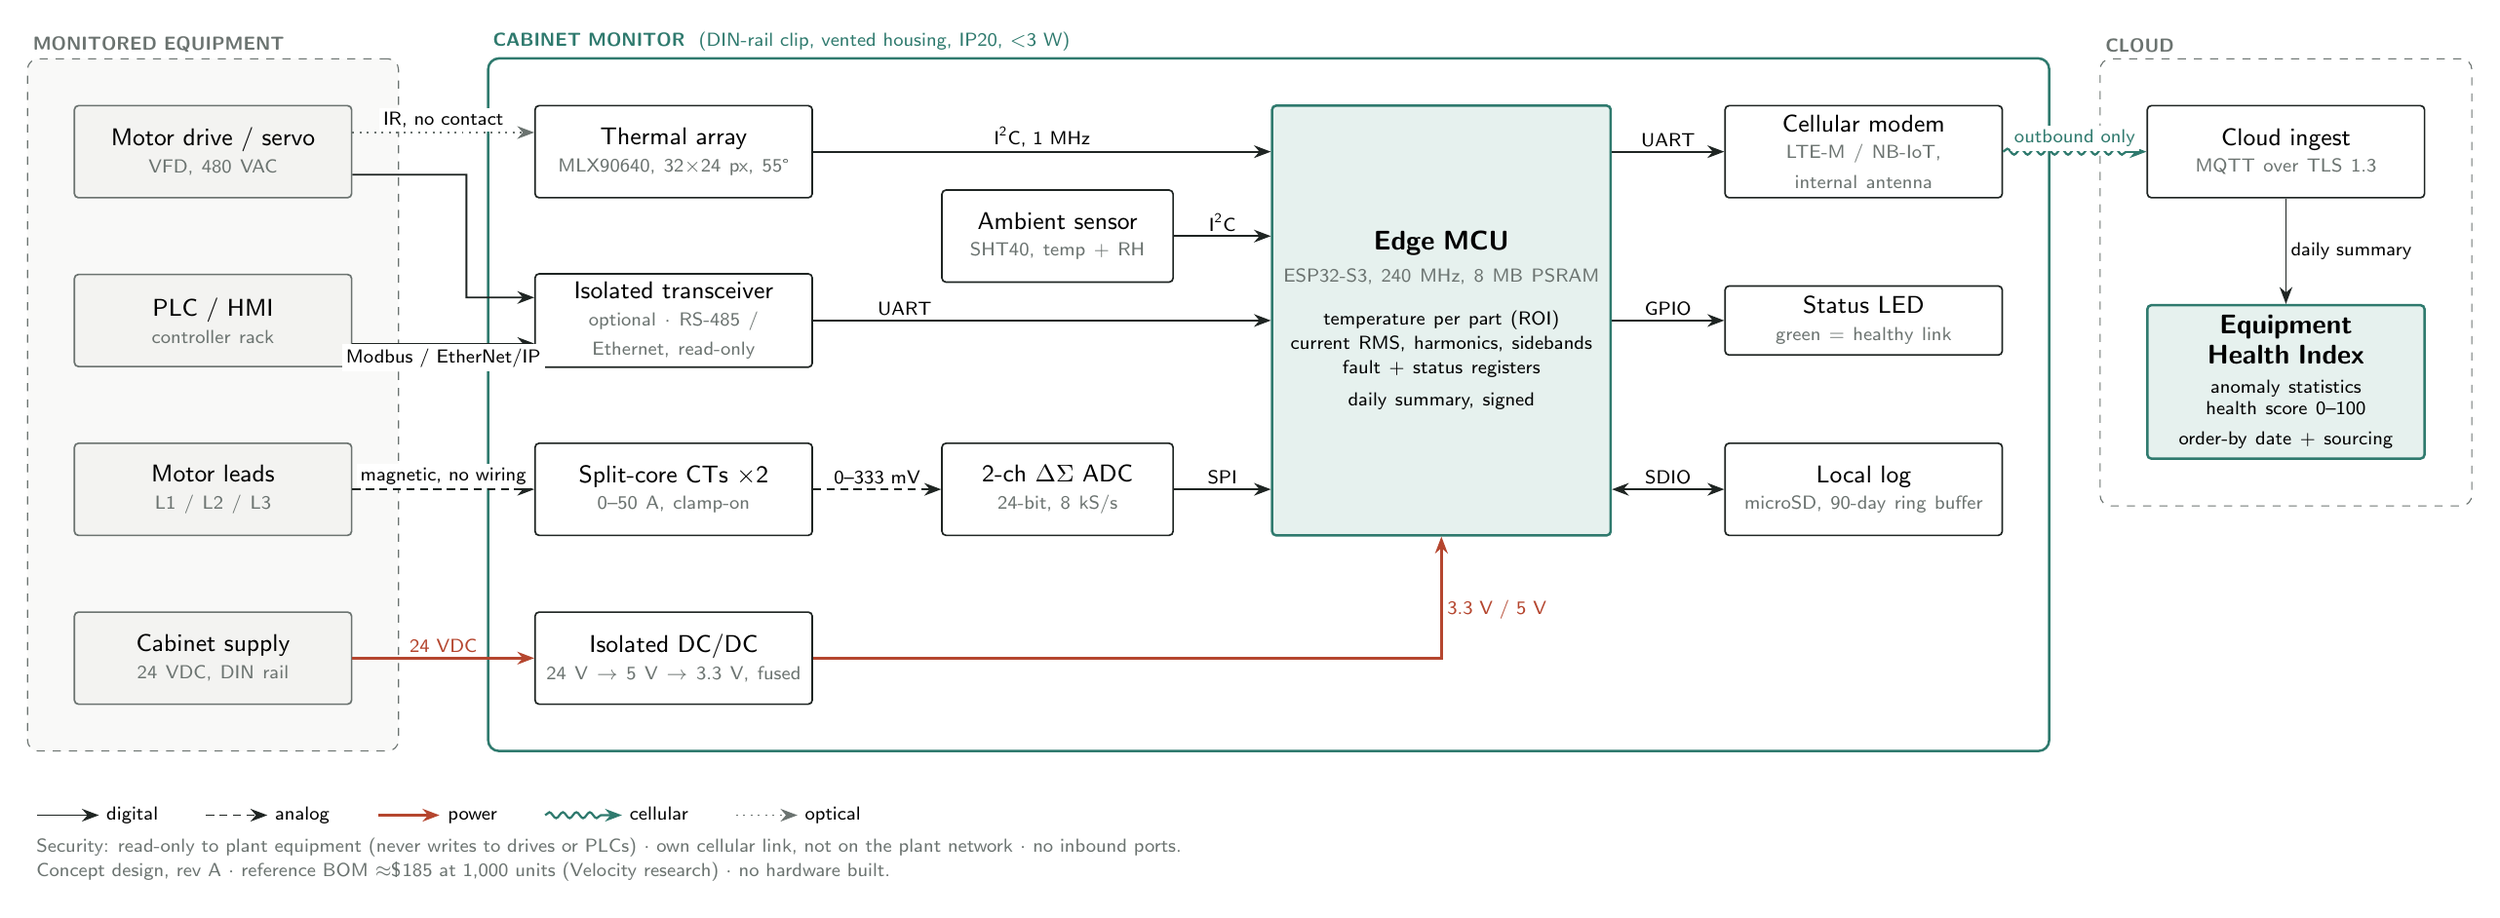
\begin{tikzpicture}

% ---------- grid ----------
% columns: field 0 | front-end 6 | conversion 11 | MCU 16 | comms 21.5 | cloud 27
% rows:    0 | -2.2 | -4.4 | -6.6

% monitored equipment
\node[ext] (drive) at (0,0)    {Motor drive / servo\sub{VFD, 480 VAC}};
\node[ext] (plc)   at (0,-2.2) {PLC / HMI\sub{controller rack}};
\node[ext] (leads) at (0,-4.4) {Motor leads\sub{L1 / L2 / L3}};
\node[ext] (psu)   at (0,-6.6) {Cabinet supply\sub{24 VDC, DIN rail}};

% sensing front end
\node[blk] (cam)  at (6,0)    {Thermal array\sub{MLX90640, 32$\times$24 px, 55\textdegree}};
\node[blk] (iso)  at (6,-2.2) {Isolated transceiver\sub{optional $\cdot$ RS-485 / Ethernet, read-only}};
\node[blk] (ct)   at (6,-4.4) {Split-core CTs $\times$2\sub{0--50 A, clamp-on}};
\node[blk] (dcdc) at (6,-6.6) {Isolated DC/DC\sub{24 V $\to$ 5 V $\to$ 3.3 V, fused}};

% conversion
\node[blk, minimum width=30mm, text width=28mm] (amb) at (11,-1.1) {Ambient sensor\sub{SHT40, temp + RH}};
\node[blk, minimum width=30mm, text width=28mm] (adc) at (11,-4.4) {2-ch $\Delta\Sigma$ ADC\sub{24-bit, 8 kS/s}};

% edge MCU (spans rows 0 .. -4.4)
\node[core, minimum width=44mm, text width=42mm, minimum height=56mm] (mcu) at (16,-2.2) {%
  {\normalsize\bfseries Edge MCU}\\[1pt]
  {\scriptsize\color{muted}ESP32-S3, 240 MHz, 8 MB PSRAM}\\[8pt]
  \scriptsize temperature per part (ROI)\\[1pt]
  \scriptsize current RMS, harmonics, sidebands\\[1pt]
  \scriptsize fault + status registers\\[1pt]
  \scriptsize daily summary, signed};

% comms + storage
\node[blk] (modem) at (21.5,0)    {Cellular modem\sub{LTE-M / NB-IoT, internal antenna}};
\node[blk] (sd)    at (21.5,-4.4) {Local log\sub{microSD, 90-day ring buffer}};
\node[blk, minimum height=9mm] (led) at (21.5,-2.2) {Status LED\sub{green = healthy link}};

% cloud
\node[blk] (ingest) at (27,0) {Cloud ingest\sub{MQTT over TLS 1.3}};
\node[core, minimum height=20mm] (xray) at (27,-3.0) {%
  {\normalsize\bfseries Equipment Health Index}\\[3pt]
  \scriptsize anomaly statistics\\[0pt]\scriptsize health score 0--100\\[0pt]\scriptsize order-by date + sourcing};

% ---------- zones (labels sit above the dashed line) ----------
\begin{scope}[on background layer]
  \node[zone, fill=field!50, fit=(drive)(psu)] (zf) {};
  \node[zone, draw=accent, solid, line width=0.9pt, fill=white, fit=(cam)(dcdc)(mcu)(modem)(sd)(led)] (zd) {};
  \node[zone, fit=(ingest)(xray)] (zc) {};
\end{scope}
\node[zonelab, text=muted]  at (zf.north west) {MONITORED EQUIPMENT};
\node[zonelab, text=accent] at (zd.north west) {\MakeUppercase{\devname}\ \ \textmd{(DIN-rail clip, vented housing, IP20, $<$3 W)}};
\node[zonelab, text=muted]  at (zc.north west) {CLOUD};

% ---------- field -> front end ----------
\draw[opt]   ($(drive.east)+(0,0.25)$) -- node[lab, above]{IR, no contact} ($(cam.west)+(0,0.25)$);
\draw[bus]   ($(drive.east)+(0,-0.3)$) -| (3.3,-1.9) -- ($(iso.west)+(0,0.3)$);
\draw[bus]   ($(plc.east)+(0,-0.3)$) -- node[lab, below]{Modbus / EtherNet/IP} ($(iso.west)+(0,-0.3)$);
\draw[ana]   (leads) -- node[lab, above]{magnetic, no wiring} (ct);
\draw[power] (psu) -- node[lab, above, text=pwr]{24 VDC} (dcdc);

% ---------- front end -> MCU ----------
\draw[bus] (cam.east) -- node[lab, above, pos=0.5]{I\textsuperscript{2}C, 1 MHz} (cam.east -| mcu.west);
\draw[bus] (amb.east) -- node[lab, above]{I\textsuperscript{2}C} (amb.east -| mcu.west);
\draw[bus] (iso.east) -- node[lab, above, pos=0.2]{UART} (iso.east -| mcu.west);
\draw[ana] (ct) -- node[lab, above]{0--333 mV} (adc);
\draw[bus] (adc.east) -- node[lab, above]{SPI} (adc.east -| mcu.west);
\draw[power] (dcdc.east) -- (16,-6.6) -- node[lab, right, text=pwr, pos=0.4]{3.3 V / 5 V} (mcu.south);

% ---------- MCU -> comms / storage ----------
\draw[bus] (modem.west -| mcu.east) -- node[lab, above]{UART} (modem.west);
\draw[bus, <->] (sd.west -| mcu.east) -- node[lab, above]{SDIO} (sd.west);
\draw[bus] (led.west -| mcu.east) -- node[lab, above]{GPIO} (led.west);

% ---------- cloud ----------
\draw[rf]  (modem) -- node[lab, above, text=accent]{outbound only} (ingest);
\draw[bus] (ingest) -- node[lab, right]{daily summary} (xray);

% ---------- legend + notes ----------
\node[anchor=north west, font=\scriptsize, align=left] at ($(zf.south west)+(0,-6mm)$) {%
  \tikz[baseline=-0.6ex]\draw[bus](0,0)--(8mm,0);\ digital \qquad
  \tikz[baseline=-0.6ex]\draw[ana](0,0)--(8mm,0);\ analog \qquad
  \tikz[baseline=-0.6ex]\draw[power](0,0)--(8mm,0);\ power \qquad
  \tikz[baseline=-0.6ex]\draw[rf](0,0)--(10mm,0);\ cellular \qquad
  \tikz[baseline=-0.6ex]\draw[opt](0,0)--(8mm,0);\ optical\\[4pt]
  {\color{muted}Security: read-only to plant equipment (never writes to drives or PLCs) $\cdot$ own cellular link, not on the plant network $\cdot$ no inbound ports.}\\[1pt]
  {\color{muted}Concept design, rev A $\cdot$ reference BOM $\approx$\$185 at 1{,}000 units (Velocity research) $\cdot$ no hardware built.}};

\end{tikzpicture}
\end{document}
